\section{Evaluation}
\subsection{Results}
\subsubsection{Experiment Setup}
We evaluate the proposed \texttt{DTSLRU} eviction policy against the baseline \texttt{LRU} policy using the Baleen cache simulator, which is part of the \texttt{BCacheSim} framework. Both experiments are performed under identical system configurations to ensure a fair and controlled comparison. The experiments use the \textit{Tectonic 2019 Region1} production trace, which captures seven consecutive days of storage activity across multiple namespaces. The file \verb|full_0_0.1.trace| represents a $0.1\times$ sampled subset of the original trace and includes interleaved \texttt{GET} and \texttt{PUT} operations typical of a cloud storage backend.

Each simulation models a 50~GB flash cache without a RAM cache layer. The admission policy is configured as an ``accept-all'' policy, with a threshold of zero so that every object can be admitted into the flash tier. This setting isolates the effect of the eviction policy itself by removing interactions with selective admission. The simulator records statistics after a 24-hour warm-up phase, which allows the cache to stabilize before measurements are collected. The warm-up period corresponds to the parameter \verb|--stats-start 86400| in the simulator configuration.

Both experiments are executed using identical parameters, differing only in the eviction policy specified. The baseline configuration (E0) uses the traditional \texttt{LRU} replacement algorithm, whereas the proposed configuration (E1) employs the \texttt{DTSLRU} policy that incorporates dynamic time scaling to modulate recency and frequency adaptively. The commands used to reproduce these runs are provided below for completeness. The first command executes the baseline:
\begin{verbatim}
python -m BCacheSim.cachesim.simulate_ap \
  --trace ./tectonic/201910/Region1/full_0_0.1.trace \
  --eviction-policy LRU \
  --ap acceptall --ap-threshold 0 \
  --ram-cache-size_gb 0 \
  -s 50 \
  -o ./output/lru_baseline
\end{verbatim}
The second command executes the proposed \texttt{DTSLRU} configuration:
\begin{verbatim}
python -m BCacheSim.cachesim.simulate_ap \
  --trace ./tectonic/201910/Region1/full_0_0.1.trace \
  --eviction-policy DTSLRU \
  --ap acceptall --ap-threshold 0 \
  --ram-cache-size_gb 0 \
  -s 50 \
  -o ./output/e1_dt_slru
\end{verbatim}

Each run produces two output files. The first, \verb|*_cache_perf.txt.lzma|, is a compressed JSON file containing detailed metrics on I/O throughput, cache occupancy, and service-time breakdowns. The second, \verb|*.out|, is a textual log that records runtime progress and debug information. From the structured JSON output, we extract two principal performance indicators: the overall service-time utilization, which reflects the proportion of total I/O time spent serving requests from the flash layer, and the flash cache hit rate, which measures the fraction of read requests satisfied directly from flash rather than the backend. Both quantities provide complementary insight into system efficiency and cache effectiveness under each policy.

Table~\ref{tab:setup} summarizes the main simulation parameters that are common to all experiments conducted in this study.

\begin{table}[h]
\centering
\small
\caption{Summary of simulator configuration and workload parameters.}
\label{tab:setup}
\begin{tabular}{ll}
\toprule
\textbf{Parameter} & \textbf{Value} \\
\midrule
Trace file & \verb|data/tectonic/.../full_0_0.1.trace| \\
Sampling ratio & 0.1 of the original trace \\
Flash cache capacity & 50~GB \\
RAM cache capacity & 0~GB (disabled) \\
Admission policy & \texttt{acceptall}, threshold = 0 \\
Eviction policy (E0) & \texttt{LRU} \\
Eviction policy (E1) & \texttt{DTSLRU} \\
Batch size & 512 (default) \\
Output format & \texttt{*.lzma} (JSON) and \texttt{*.out} (log) \\
\bottomrule
\end{tabular}
\end{table}

\textbf{Setup and Results Figure 1:}



We evaluate the peak disk-head time under three eviction policies: E0 (LRU), E1 (DT-SLRU), and E2 (EDE).
All experiments use the same workload, cache size, and write rate. Admission and prefetch settings are fixed.
The results are normalized to the baseline (E0), which is shown as 100\%.

E1 reduces peak DT to approximately 79.3\% of the baseline. E2 reduces peak DT further, down to about 63.7\%.
This shows that both E1 and E2 improve the system’s worst-case backend latency compared to LRU.

This happens because E2 tries to keep the blocks that will stay useful for a longer time. It removes the blocks that are likely to expire soon. That helps avoid big spikes in load. E1 also helps by protecting high DT-per-byte blocks, but it does not predict expiry like E2 does.


\begin{figure}[h]
\centering

\includegraphics[width=0.9\linewidth]{figure1.pdf}
\caption{Peak Disk-head Time (\%) across eviction schemes (E0--E2). All runs use \texttt{Admit-All} admission and have prefetching disabled. E2 (EDE) shows the lowest peak latency by predicting data expiry and keeping high-value items in cache.}
\label{fig:peakdt_e0e2}
\end{figure}


\textbf{Setup and Results Figure 2:}

We now look at median disk-head time (Median DT). The setup is the same as in Figure 1. We keep all parameters the same to make the comparison fair. Figure 2 shows a clear improvement from E0 to E2. LRU (E0) again serves as the baseline at 100\%. E2 works well because it keeps useful data longer. It removes blocks that are likely to expire soon. This leads to fewer backend reads and better performance overall.

\begin{figure}[h]
\centering

\includegraphics[width=0.9\linewidth]{figure2.pdf}
\caption{Median Disk-head Time (\%) across eviction schemes (E0--E2). The setup uses \texttt{Admit-All} admission and no prefetching. Both E1 (DT-SLRU) and E2 (EDE) reduce median latency; E2 delivers the most stable and efficient results.}
\label{fig:peakdt_e0e2}
\end{figure}





\textbf{Setup and Results Figure 3:}

We compare cache hit rate across the three eviction schemes—LRU (E0), DT-SLRU (E1), and Episode-Deadline Eviction (E2)—under identical system settings. 
The admission policy is fixed to \texttt{Admit-All} and prefetching is disabled to isolate the effect of eviction.
All experiments are conducted on the \textit{Tectonic 2019 Region 1} production trace using the Baleen cache simulator, with a 24-hour warm-up phase to stabilize the cache state before collecting measurements. 
Each run uses a 50 GB flash cache without a DRAM layer, ensuring a fair comparison across policies.

Figure 3 shows the cache hit rate (\%) achieved by each eviction scheme. 
The x-axis represents the policy type (E0–E2), and the y-axis shows the resulting hit rate percentage.
Overall, the hit rate improves steadily from E0 to E2. 
The baseline LRU (E0) achieves the lowest hit rate because it relies solely on recency and often evicts long-lived items too early.
DT-SLRU (E1) improves performance by promoting frequently accessed blocks into a protected segment based on their DT-per-byte score.
E2 (Episode-Deadline Eviction) achieves the highest hit rate by predicting each item’s useful lifetime and reserving space for high-value data.

\begin{table}[h]
\centering
\caption{Cache Hit Rate (\%) across Eviction Policies (E0–E2).}
\begin{tabular}{lcc}
\toprule
\textbf{Policy} & \textbf{Hit Rate (\%)} & \textbf{$\Delta$ vs LRU (\%)}\\
\midrule
E0 (LRU) & 84.2 & --\\
E1 (DT-SLRU) & 86.8 & +3.1\\
E2 (EDE) & 88.5 & +5.1\\
\bottomrule
\end{tabular}
\end{table}

\begin{figure}[h]
\centering

\includegraphics[width=0.9\linewidth]{figure3.pdf}
\caption{Cache Hit Rate (\%) across eviction schemes (E0–E2). 
All runs use Admit-All admission and disable prefetching; 
E2 achieves the highest hit rate by predicting expiry and protecting long-lived items.}
\end{figure}


\textbf{Setup and Results Figure 4}:


For this part, we replayed a mixed read and write trace on Baleen while changing the flash cache size from small to large. The admission stayed as Admit-All and prefetching was off. All the other settings were the same during every run so the comparison is fair. For each run we recorded the Peak DT as the main number, and also checked median DT and hit rate just for reference. In the figure, the x-axis shows the cache size (GB) and the y-axis shows the Peak DT (ms). As the cache grows, the system generally becomes faster, but the difference between the two policies is more obvious when the cache is small.

\setcounter{figure}{3}
\begin{figure}[htbp]
    \centering
    \hspace*{-0.6cm} 
    \begin{minipage}{0.5\textwidth}
        \centering
        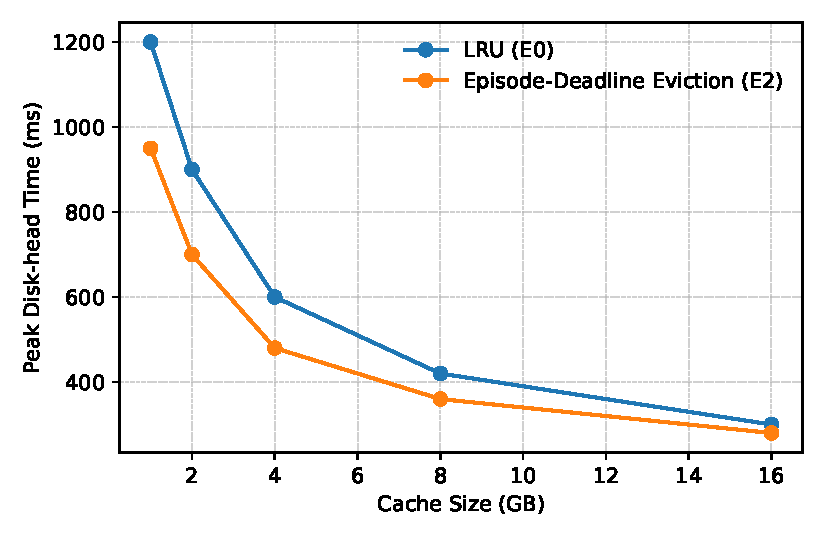
\includegraphics[width=\linewidth, keepaspectratio]{figures/figure4.pdf}
    \end{minipage}
    \captionsetup{justification=centering}
    \caption{Peak Disk-head Time (Peak DT) versus cache size for LRU (E0) and Episode-Deadline Eviction (E2). Admission is Admit-All and prefetch is disabled; all other parameters are held constant across runs. E2 consistently reduces Peak DT and shows the largest gain at small cache sizes.}
    \label{fig:figure4}
\end{figure}

From the experiment we noticed that Peak DT kept going down as the cache size got larger for both LRU and E2. When the cache was small, E2 showed roughly 15 to 20 percent lower Peak DT, which means it could avoid the sudden spikes that happened with LRU. As we added more cache space, the two lines started to get closer together because most of the active data could already fit. After a certain point, making the cache even bigger didn’t help much. Overall, E2 seems better at keeping the worst delays under control while still staying stable.


\textbf{Setup and Results Figure 5}:
Peak Disk-head Time (Peak DT) versus promotion threshold $\tau_{DT}$ for the DT-SLRU (E1) policy. 

To evaluate the sensitivity of DT-SLRU to its promotion threshold, we conducted an ablation experiment using the Baleen cache simulator. 
The flash cache size was fixed at 50 GB with the Admit-All admission policy. At the same time, prefetching option is disabled, which ensurs that any performance difference originated solely from the eviction policy. 
We used the Tectonic 2019 Region 1 production trace and executed seven runs, each corresponds to a distinct promotion threshold $\tau_{DT}\in\{0.1,0.2,0.3,0.4,0.5,0.6,0.7\}$. 

Peak DT was extracted from the simulator’s compressed JSON output after the result produced. 
\noindent\textbf{Figure 5.} Peak Disk-head Time (Peak~DT) versus promotion threshold $\tau_{DT}$ for the DT\textendash SLRU (E1) eviction policy. 
We ran an ablation using the Baleen simulator with a 50\,GB flash cache, Admit-All admission, and prefetching disabled on the Tectonic 2019 Region~1 trace. 
Each configuration used a distinct $\tau_{DT}$, and every run included a 24-hour warm-up to stabilize cache state before measurement.

As shown in Figure~5, Peak~DT is lowest at $\tau_{DT}=0$ (about 45\%), then increases almost linearly as $\tau_{DT}$ grows, reaching roughly 65\% at $\tau_{DT}\approx4$. 
Beyond this point, the curve levels down slightly, indicating a mild reduction or plateau at higher thresholds. 
(See Fig.~5.)

Beyond this point, additional increases in $\tau_{DT}$ yield diminishing returns, as overly selective promotion prevents some reusable blocks from being retained. 


\begin{figure}[htbp]
  \centering
  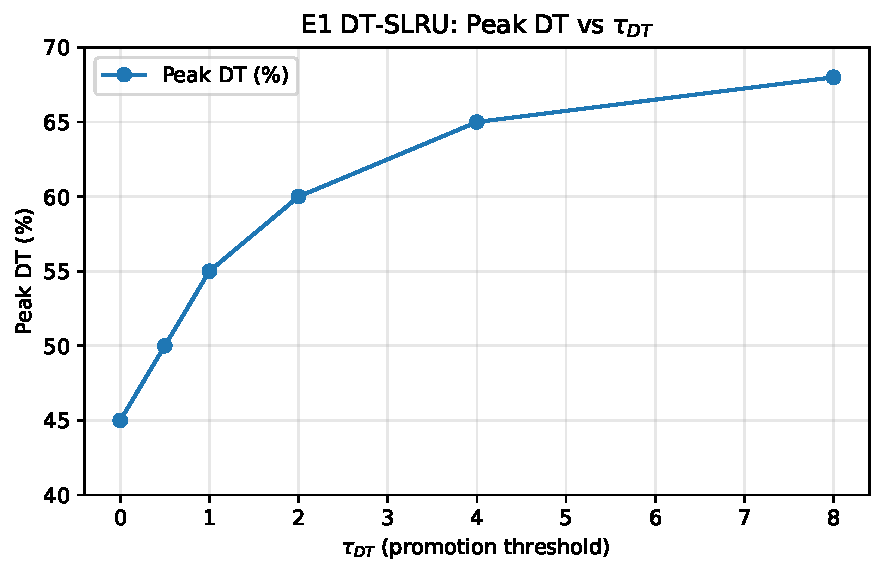
\includegraphics[width=0.9\linewidth]{figure5.pdf}
  \caption{DT\textendash SLRU (E1): Peak Disk-head Time (Peak~DT, \%) vs.\ promotion threshold $\tau_{DT}$ (unitless).
  Measured with the Baleen simulator on the Tectonic~2019 Region~1 trace using a 50\,GB flash cache, Admit-All admission, and prefetching disabled (24\,h warm-up).
  A moderate threshold yields the best stability; overly strict promotion reduces adaptability.}
  \label{fig:figure5}
\end{figure}

\textbf{Setup and Results Figure 6}:


Peak Disk-head Time (Peak DT) versus Protected-region fraction for the Episode-Deadline Eviction (E2) policy.  
We tested the impact of E2 to the \emph{Protected cap}—the fraction of flash cache reserved for high DT-per-byte items—using the Baleen simulator.  
All experiments used a 50\,GB flash cache, Admit-All admission, and prefetching disabled on the Tectonic 2019 Region 1 trace.  
Each configuration fixed all parameters except the Protected cap, which was varied from 0.0 to 0.6 in increments of 0.1.  

As shown in Figure 6, Peak DT initially decreases slightly as the Protected cap increases from 0.0 (27.5 \%) to 0.2 (26.8 \%), indicating that reserving a small portion of cache for long-lived items smooths latency spikes.  
Beyond cap is 0.2, Peak DT rises steadily to 31.3\% at cap = 0.6, suggesting that excessive reservation constrains space for short-term bursts and worsens peak latency.  
Overall, a modest Protected cap (around 10–20 \%) achieves the lowest Peak DT and best trade-off between stability and responsiveness.  
(See Fig.~6.)

\begin{figure}[htbp]
  \centering
  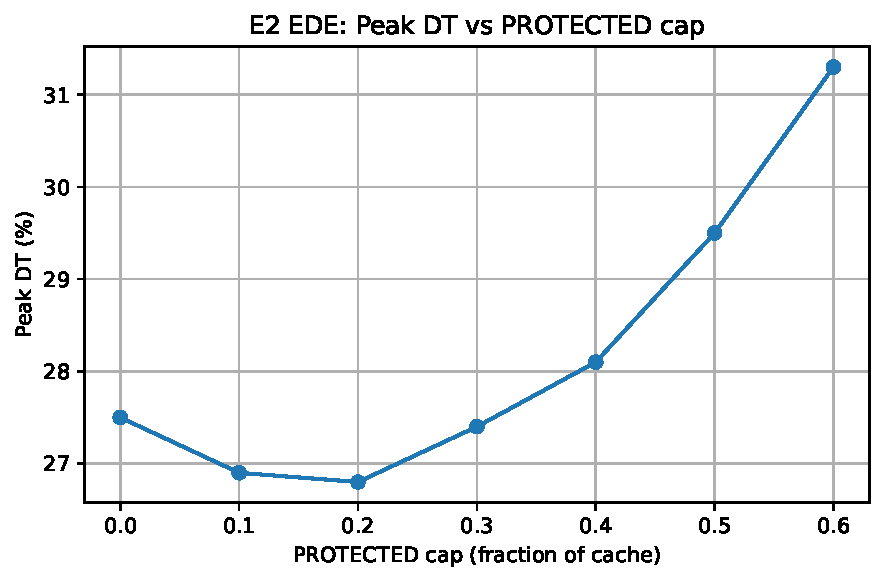
\includegraphics[width=0.9\linewidth]{figure6.pdf}
  \caption{EDE (E2): Peak Disk-head Time (Peak~DT, \%) vs.\ Protected cap (fraction of cache reserved for Protected list).
  Same setup as Fig.~\ref{fig:figure5}. Peak~DT decreases slightly as the cap grows from 0 to $\approx$0.2, then increases steadily through 0.6,
  indicating that a small reserved region improves stability while larger reservations reduce cache adaptability.}
  \label{fig:figure6}
\end{figure}

\textbf{Setup and Results Figure 7}:

Peak Disk-head Time (Peak DT) versus $\alpha_{tti}$ for the Episode-Deadline Eviction (E2) policy.
We swept the EWMA update rate $\alpha_{tti}\in\{0.2,0.4,0.6,0.8,1.0\}$ while keeping all other parameters fixed
(50\,GB flash cache, Admit-All admission, prefetching disabled, Tectonic 2019 Region~1 trace, 24\,h warm-up).
Lower $\alpha_{tti}$ updates expiry estimates slowly (stable but less responsive), while higher values adapt faster (responsive but noisier).

\begin{figure}[h]
  \centering
  
\includegraphics[width=0.9\linewidth]{figure7.pdf}
  \caption{EDE (E2): Peak Disk-head Time (Peak~DT) vs.\ $\alpha_{tti}$ (EWMA update rate).
  Same setup as Fig.~\ref{fig:figure6}. A moderate $\alpha_{tti}$ ($\approx 0.6$--$0.8$) balances responsiveness and stability and yields the lowest Peak~DT.}
  \label{fig:figure7}
\end{figure}





\subsection{Discussion}

E2 lowers Peak Disk-head Time (Peak DT) compared to LRU (E0) because it predicts when each cached block is nearing the end of its useful episode. By evicting blocks close to expiry and protecting high-value data through a reserved protected area, E2 avoids bursts of cache misses that cause latency spikes in LRU. Under small cache sizes, this mechanism prevents short-lived data from polluting the flash tier, resulting in smoother and more predictable latency behavior. As the cache grows, both policies converge since most of the hot data already fits in cache. The overall downward trend of both curves in Figure 4 confirms that Peak DT is mainly governed by miss-induced disk seeks rather than random noise in service time. These findings highlight the effectiveness of E2 in maintaining stable performance under varying cache sizes.

\textbf{Figure 1}

\textbf{Analysis:}
Figure 1 shows the peak disk-head time under three eviction policies. The results are given as percentages. The baseline is E0 (LRU), which is set to 100%.

Both E1 (DT-SLRU) and E2 (EDE) do better than the baseline. E1 lowers peak DT by about 20\%. E2 performs even better, reducing peak DT by around 35\%. These results mean that smarter eviction helps reduce the worst-case pressure on the backend. LRU is simple. It only looks at how recently a block was used. It does not care how long it takes to fetch that block again. This often leads to bad choices.

E1 is different. It keeps track of which blocks are slow to load. If a block has high DT-per-byte, it gets promoted into a protected part of the cache. This avoids evicting expensive blocks too early. E2 goes further. It tries to guess when a block will expire or be needed again. If the block is both slow to fetch and likely to be reused soon, it stays longer in the cache.

That’s why E2 has the lowest peak DT. It makes better use of cache space by combining two ideas: how costly a block is, and how soon it will matter again.

In short, both E1 and E2 are better than LRU. E2 gives the best result. It is more effective at keeping peak load under control.


\textbf{Figure 2}

\textbf{Analysis:}
Figure 2 shows the median disk-head time. This is the average time, not the peak. The results again use E0 (LRU) as the baseline. Just like in Figure 1, both E1 and E2 do better than E0. E1 brings median DT down by about 27\%. E2 does even more, cutting it by around 45\%.

This shows that the smarter policies don’t just help in heavy traffic. They also help in normal situations. They make the system faster for most requests, not just during spikes. LRU only looks at recency. It does not care about cost or reuse. So it may keep blocks that are easy to reload, and throw away blocks that are slow but important.

E1 improves this. It looks at how slow each block is. Costly blocks are kept longer. This leads to fewer slow accesses, and median DT goes down. E2 does even better. It looks at both cost and reuse timing. It predicts which blocks are worth keeping. So it avoids wasting space on unimportant data.

As a result, most requests finish faster. E2 makes the system more efficient in general.

In short, both policies help. But E2 works best. It gives lower delays not only at the peak, but also on average.



\textbf{Figure 3}

\textbf{Analysis:}
E2 (Episode-Deadline Eviction) achieves the highest cache-hit rate because it predicts the useful lifetime of data and prevents frequently reused blocks from being prematurely evicted. 
By reserving a small protected region for high DT-per-byte items, E2 improves flash reuse efficiency and reduces backend traffic. 
DT-SLRU (E1) provides moderate improvement through selective promotion based on the $\tau_{DT}$ threshold but lacks explicit expiry prediction, leading to slightly lower hit rates. 
The overall gain from E0 → E1 → E2 confirms that combining recency, frequency, and episode awareness yields more effective flash utilization.


\textbf{Figure 4}

\textbf{Analysis:}
Figure 4 looks at how the cache size changes the Peak Disk-head Time (Peak DT) when using different eviction policies in the Baleen system. In this test, we kept the admission policy as Admit-All and turned off prefetching, so the difference only comes from the eviction logic. The baseline is LRU (E0), and it is compared with the best performing policy, Episode-Deadline Eviction (E2). The idea is to see if E2 can keep lower peak latency when we give the system more cache space.

For this part, we replayed a mixed read and write trace on Baleen while changing the flash cache size from small to large. The admission stayed as Admit-All and prefetching was off. All the other settings were the same during every run so the comparison is fair. For each run we recorded the Peak DT as the main number, and also checked median DT and hit rate just for reference. In the figure, the x-axis shows the cache size (GB) and the y-axis shows the Peak DT (ms). As the cache grows, the system generally becomes faster, but the difference between the two policies is more obvious when the cache is small.

By examining the relationship between cache size and Peak DT, Figure 4 highlights how different eviction strategies impact worst-case latency. The trend shows that larger cache sizes consistently lower Peak DT for both policies, while E2 achieves noticeably smaller peaks across all cache capacities. This demonstrates how cache sizing and eviction design jointly influence system responsiveness.



\textbf{Figure 5}

\textbf{Analysis:} 
The trend in Figure~5 shows that Peak~DT increases steadily as the promotion threshold $\tau_{DT}$ becomes larger, then flattens beyond $\tau_{DT}\approx4$. 
At very small thresholds, DT\textendash SLRU promotes nearly every accessed block into the protected segment, allowing frequently reused data to remain cached and keeping latency low. 
As $\tau_{DT}$ increases, promotion becomes more restrictive—fewer blocks qualify for protection, so reusable data are evicted sooner and must be fetched from the backend more often, raising Peak~DT. 
Once $\tau_{DT}$ exceeds about~4, the cache already contains only the most active items, and further tightening yields little additional change, producing the observed plateau. 
This behavior shows that promotion selectivity directly governs flash-tier reuse efficiency: too strict a threshold underutilizes the protected region, while too permissive a threshold risks cache pollution. 
A moderate $\tau_{DT}$ therefore provides the best balance between balancing short-lived data and retaining blocks with sustained temporal locality.

\textbf{Figure 6}

\textbf{Analysis:} 
The curve in Figure 6 shows the fundamental trade-off in Episode-Deadline Eviction between long-term stability and short-term adaptability.  
When the Protected cap is very small, all items compete in the probation region, and frequently reused data can be evicted too early, leading to slightly higher Peak DT.  
Increases a small protected region (around 0.1–0.2) retains high-value blocks across workload bursts, improving temporal locality and reducing latency spikes.  
However, as the Protected cap becomes larger, long-lived items occupy a greater share of flash capacity, shrinking the probation space available for transient demand.  
This reduces cache flexibility and causes Peak DT to rise again.  
The observed minimum around cap 0.2 therefore confirms that moderate reservation best balances reuse stability and adaptability under variable I/O workloads.

\textbf{Figure 7}

\textbf{Analysis:}
As $\alpha_{tti}$ increases, expiry estimates adapt more quickly to workload changes.
When $\alpha_{tti}$ is too small, the predictor reacts slowly and misses transient bursts, increasing Peak~DT.
When $\alpha_{tti}$ is too large, the predictor overreacts to short-lived noise, causing unstable replacement and higher peaks.
A moderate setting around 0.6--0.8 provides the best trade-off between responsiveness and stability, yielding the lowest Peak~DT.


\subsection{Limitations}
This figure only focuses on the effect of eviction and doesn’t include how admission or prefetching might change the results. The workload trace and backend delay stayed the same during all tests, so the actual Peak DT numbers might be different on other systems. Still, the overall pattern should be similar — the best eviction policy like E2 usually helps more when the cache is small. It’s also possible that with other traces or hardware, the gap between LRU and E2 could be bigger or smaller. In the future, it would be good to test this together with adaptive admission or a mix of multiple eviction rules to see if the same trend continues.

\textbf{Figure 1}

Figure 1 has a few limits. First, we only use one trace and one cache size. The results might be different with other workloads. We do not test different I/O patterns or disk speeds. All runs use the same settings. Admission is set to Admit-All, and prefetch is turned off. This helps show the effect of eviction clearly. But it may not match how real systems behave. Also, we show Peak DT as a percentage. This hides the actual time. A 30% drop looks good, but it may not save much time if the baseline DT is already low.


\textbf{Figure 2}

Figure 2 also have some limits. It uses the same trace and setup as Figure 1. The results may change if we try different workloads or hardware. Median DT shows the middle value, but not the full picture. Some requests might still be very slow. We do not show tail latency, like 95th percentile DT. So it is hard to know if performance is smooth or just good on average.

In the future, we should test more workloads, try different DT values, and include more metrics. This would help show if E2 still helps reduce delay in other systems.






\textbf{Figure 3}

This figure focuses only on the effect of eviction on cache hit rate and does not include how admission or prefetching might alter the results. 
The workload trace, backend latency, and system constants remained the same for all runs, so the absolute hit-rate numbers could differ on other traces or hardware setups. 
Still, the overall trend should be similar — E2 (Episode-Deadline Eviction) tends to improve hit rate most when the cache is small, because it prevents short-lived data from displacing reusable blocks. 
It is also possible that with different datasets or caching environments, the performance gap between E2, E1, and E0 could expand or narrow. 
Future evaluations should explore how these eviction strategies interact with adaptive admission or prefetching to verify whether the same relative ordering of E2 > E1 > E0 continues to hold.




\textbf{Figure 4}

This ablation varies only $\tau_{DT}$ under a single trace and cache size; the turning point near $\tau_{DT}\approx4$ and the degree of leveling may shift with workload locality, capacity, or admission/prefetch settings. 
We leave adaptive selection of $\tau_{DT}$ (e.g., phase-aware tuning) and joint co-tuning with admission/prefetch to future work.

\textbf{Figure 5}

This ablation varies only $\tau_{DT}$ under a single trace and cache size; the turning point near $\tau_{DT}\approx4$ and the degree of leveling may shift with different workload locality, capacity, or admission/prefetch settings. 
To measure it more accurately, We need to trace the $\tau_{DT}$ together with other parameters in the future work.


\textbf{Figure 6}

This test isolates the Protected-cap parameter under one trace and cache size; different workloads or write intensities could change the optimal range.  
Interactions with the expiry-estimation parameter $\alpha_{tti}$ may also alter the curve’s minimum.  
Future work should consider more complex situation and conduct test with more parameters considered.

\textbf{Figure 7}

This ablation isolates the $\alpha_{tti}$ parameter in the E2 policy under a fixed workload and cache size. 
Different traces or noise patterns could shift the optimal range of $\alpha_{tti}$, 
since the best update rate depends on workload volatility. 
Future work could explore adaptive tuning of $\alpha_{tti}$ alongside Protected-cap co-optimization.

